\documentclass[11pt]{article}
\usepackage{fullpage}
\usepackage{amssymb}
\usepackage{amsfonts}
\usepackage{amsmath}
\usepackage{color}
\usepackage{hyperref}
\usepackage{listings}
\usepackage{graphicx}

\def\QU{{\sf QU}$\,$}

\title{User Manual for {\QU}\\v. 1.0}

\author{Pietro Longhi\\\href{mailto:pietro.longhi@gmail.com}{pietro.longhi@gmail.com} }












\begin{document}

\maketitle
\abstract{
A short manual for using the software \QU to produce generating series of 2d-4d framed BPS degeneracies with spin, to  compute BPS monodromies from graphs.
}
%%%%%%%%%%%%%%%%%%%%%%%%%%%%%%%%%%%%
\section{Prerequisites}
%%%%%%%%%%%%%%%%%%%%%%%%%%%%%%%%%%%%
Running \QU requires python 2.7, which can be downloaded for Windows, Mac OS and Linux at this link: \url{https://www.python.org/downloads/release/python-278/}.
Note that Linux and Moc OS likely often existing python distributions, which may be sufficient for running \QU.


%%%%%%%%%%%%%%%%%%%%%%%%%%%%%%%%%%%%
\section{Graphical interface}
%%%%%%%%%%%%%%%%%%%%%%%%%%%%%%%%%%%%
\QU comes with an elementary graphical user interface, providing the most basic functionalities. 
To launch the user interface open a terminal, navigate to the folder where \QU is located, and execute the command
\begin{lstlisting}[language=bash]
  $ python gui.py
\end{lstlisting}
This will open a window like the one shown in figure below
\begin{center}
\includegraphics[width=0.25\textwidth]{gui.png}
\end{center}
Clicking on the button {\sf Load configuration} will open a window which allows to select a configuration file, containing topological data of the graph (we explain how to prepare such a file in the next section, some examples are provided in the sub-folder {\sf graph\_data}).
\begin{center}
\includegraphics[width=0.65\textwidth]{choose-file.png}
\end{center}
Select a configuration file, for example {\sf argyres\_douglas\_3.ini}, and click {\sf Open}.
This will bring back the former window, now click on {\sf Compute and Save Soliton Data}, and select a place to save the data that will be produced, for example {\sf  argyres\_douglas\_3.txt}.

\medskip

\QU will now compute generating functions $Q^{\pm}(p,y)$ defined in the paper ``Wall crossing invariants from Spectral Networks'' by the author.
The output will be printed in the file specified in the last step above, in our example this is the file {\sf  argyres\_douglas\_3.txt} in the folder {\sf results}.
If the configuration file of the network is formatted correctly, a message similar to the following message will be printed at the top of the output file:

\medskip

\noindent \texttt{All streets have two well-defined endpoints.}\\
\texttt{All joints are of a well-defined type.}\\
\texttt{All homology classes are well-defined.}\\

\medskip

Shortly below this message a short dictionary between variables and homology classes will be printed:

\medskip

\noindent \texttt{Dictionary of formal variables and homology basis:}\\
\texttt{gamma\_1 ---> X1}\\
\texttt{gamma\_2 ---> X2}

\medskip

The data will be contained under the section {\sf SOLITON DATA}, for example

\medskip


\noindent\texttt{===============}\\
\texttt{SOLITON DATA}\\
\texttt{===============}

\smallskip

\noindent\texttt{Data of street p\_2}\\
\texttt{In american resolution}\\
\texttt{----------------------------}

\smallskip

\noindent\texttt{4d Soliton generating function (with spin)}\\
\texttt{X2/y + 1}



\bigskip

\noindent\texttt{Data of street p\_1}\\
\texttt{In american resolution}\\
\texttt{----------------------------}

\smallskip

\noindent\texttt{4d Soliton generating function (with spin)}\\
\texttt{X1*X2/y + X1/y + 1}

\medskip

et cetera. The data should be read according to the dictionary printed above. For example, in the language of the paper ``Wall crossing invariants from spectral networks'', this means that 
\begin{equation}
\begin{split}
	Q^{(+)}(p_1,y) & = 1+y^{-1} \, {\hat Y}_{\tilde\gamma_1} + y^{-1} {\hat Y}_{\tilde\gamma_1+\tilde\gamma_2} \,,\\
	Q^{(+)}(p_2,y) & = 1+y^{-1} \, {\hat Y}_{\tilde\gamma_2} \,.
\end{split}
\end{equation}
Note an important point on conventions: the monomial {\texttt{X1*X2}} does \emph{not} correspond to ${\hat Y}_{\tilde\gamma_1}{\hat Y}_{\tilde\gamma_2}$, but to ${\hat Y}_{\tilde\gamma_1+\tilde\gamma_2}$! 


%%%%%%%%%%%%%%%%%%%%%%%%%%%%%%%%%%%%
\section{Constructing a graph}
%%%%%%%%%%%%%%%%%%%%%%%%%%%%%%%%%%%%

The critical graph ${\cal W}_c$ is given to \QU by writing a text file which must be saved with the {\sf .ini} extension.
Several templates are included in the folder {\sf graph\_data}. The basic structure of the file includes two sections: {\sf Network Data} and {\sf Computation Parameters}.
For example, the file {\sf 1-herd.ini} reads

\medskip

\noindent\texttt{[Network Data]}\\

\noindent\texttt{{streets = ['p\_1','p\_2','q\_1','q\_2']}}

\noindent\texttt{branch\_points = \{}\\
\noindent\texttt{ \hspace*{10pt} 'b\_1' : ['p\_1'],}\\
\noindent\texttt{ \hspace*{10pt} 'b\_2' : ['q\_1'],}\\
\noindent\texttt{ \hspace*{10pt} 'b\_3' : ['p\_2'],}\\
\noindent\texttt{ \hspace*{10pt} 'b\_4' : ['q\_2']\}}\\

\noindent\texttt{joints = \{}\\
\noindent\texttt{ \hspace*{10pt} 'j\_1': ['p\_1', None, 'q\_1', 'p\_2', None, 'q\_2' ]\}}\\

\noindent\texttt{homology\_classes = \{}\\
\noindent\texttt{ \hspace*{10pt} 'gamma\_1' : ['p\_1', 'p\_2'],}\\
\noindent\texttt{ \hspace*{10pt} 'gamma\_2' : ['q\_1', 'q\_2'],\}}\\

\smallskip

\noindent\texttt{[Computation Parameters]}\\

\noindent\texttt{iterations = 10}

\medskip

This corresponds to the graph shown in figure below
\begin{center}
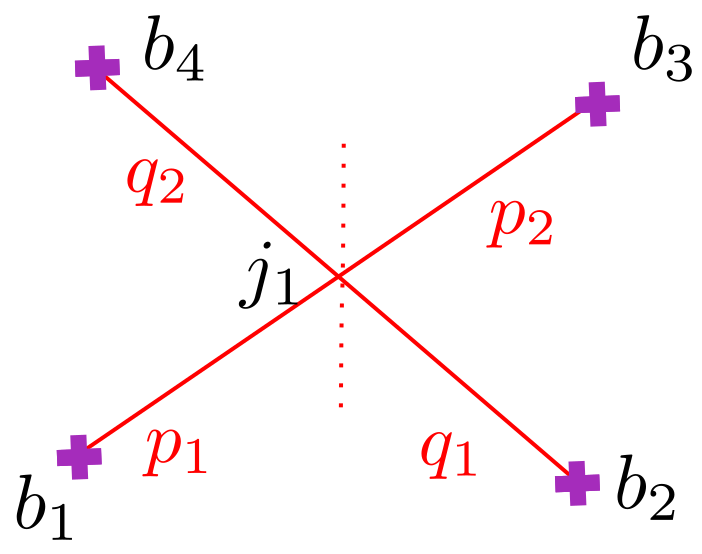
\includegraphics[width=0.25\textwidth]{1-herd.pdf}
\end{center}

\begin{itemize}

\item In {\sf streets} one must specify a list of labels for streets, the list is delimited by \emph{square brackets}, and each name is delimited by single quotation marks. 

\smallskip

\item Then one specifies a list of {\sf branch points}: this is delimited by \emph{curly brackets}, each entry is of the form

 \hspace*{10pt} {\texttt{'label' : ['street\_1', 'street\_2', 'street\_3'],}}
 
 where the first entry is a label for the branch point, the separator is a \emph{colon}, and the second entry is a list in \emph{square brackets}, containing up to three labels of edges which end on the branch point. The ordering from left to right corresponds to going \emph{counterclockwise} around the branch point.
 
 \smallskip
 
\item  Then one specifies {\sf joints}, the structure is identical to that of branch points, except that the labels of edges ending on a joint are contained in a list of up to six elements. {Important:} if there is an empty slot between two edges anding at the joint, this must be specified! In the empty slot one must write {\texttt{None}}, see the example given above.

\smallskip

\item The last field is that of {\texttt{homology\_classes}}. As the name suggests, this tells \QU which streets lift to form a homology class. 
In the example, the lift of streets $p_1$ and $p_2$ corresponds to a cycle in homology class $\gamma_1$. This is specified by adding to the list the entry

\noindent\texttt{ \hspace*{10pt} 'gamma\_1' : ['p\_1', 'p\_2'],}

with the labels of the two streets $p_1$ and $p_2$. Again it is important to note that the overall delimiters of the list are curly brackets, while the delimiters of the sub-list of street labels are square brackets, the separator is a colon.

\smallskip

\item Finally, in the section {\sf Computation Parameters} one specifies how many iterations of equation solving \QU should attempt to do, by giving a positive integer.
\end{itemize}

\end{document}





